\section{Clickstream data: Interface reduces edit distance in long surveys}
\label[SSE]{dist}
To address the research question of whether interfaces and options influenced survey response behaviors~(\textbf{RQ3}) and to explore possible reasons why participants in the long text interface exhibited lower cognitive load, we investigated differences in voting behaviors. All analyzed data are publicly available\footnote{link-to-github} for transparency and to facilitate further research. In this section, we focus on how far apart participants moved between vote updates, we call this edit distance. For example, if a participant updated their vote on the second option and then skipped three options before making their next update on the fifth option, this is an edit distance of 3. This measure helps us understand ~\textit{how} participants engaged with the survey options. We modeled three aspects of this measure: the edit distance per option, the edit distance per action, and the cumulative edit distance throughout the survey.

\begin{figure}[ht]
    \centering
    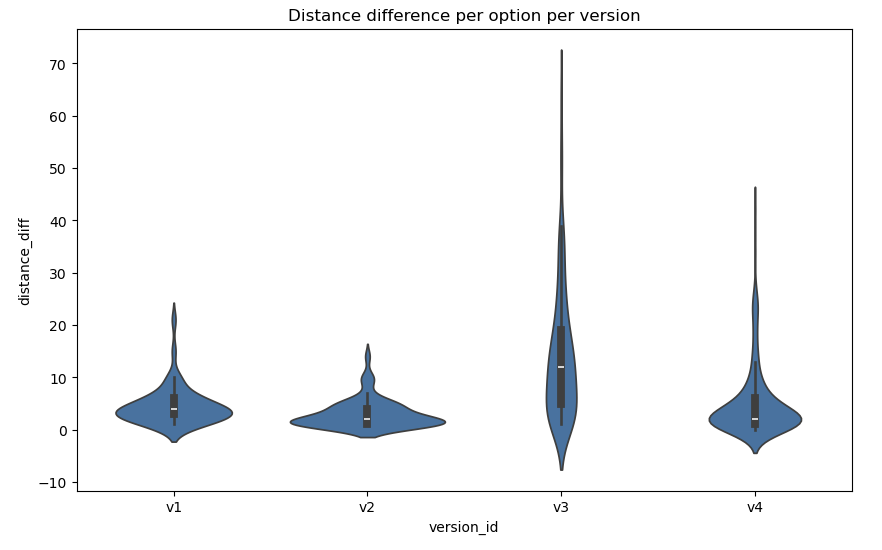
\includegraphics[width=0.65\textwidth]{content/image/distance/edit_dist_per_option.png}
    \caption{Edit Distance Per Option}
    \label{fig:dist_per_option}
\end{figure}

Edit distance per option refers to the total distance a participant moved to complete all vote adjustments for each option (Fig~\ref{fig:dist_per_option}). The figure showed that the long text interface on average had an higher edit distance with a larger spread. We constructed a hierarchical regression bayesian model that estimated a linear predictor of voting distances with the length, interface, their interaction effect and individual users as experiment variables. We present details of the model with pairwise results for brevity in Appendix XX. Our model showed significant differences, in Bayesian terms referring to a 94\% HDI not including zero, between the short and long static interfaces (mode difference of 8.5 with a 94\% HDI of [5.4, 12.0] and a large effect size of 0.94) and between the long text and long two-phase interfaces (mode difference of 8.5 with a 94\% HDI of [6.0, 12.5] and a large effect size of 0.94). Our results also show that within the short survey, there is a trend in reduction in steps between two phase interface and the text interface (75.4\% probability with a mode of 1.9 and a small effect size of 0.18), as well as a small increase between short and long two-phase versions (84.2\% probability with a mode of 1.8 and a small effect size of 0.2). While it is not surprising that the length of the survey adds to edit distances, the organizational phase reduces the need for participants to move as much to complete their votes. It also demonstrates that the two-phase interface mitigated the increase in edit distance required by participants.

\begin{figure}[ht]
    \centering
    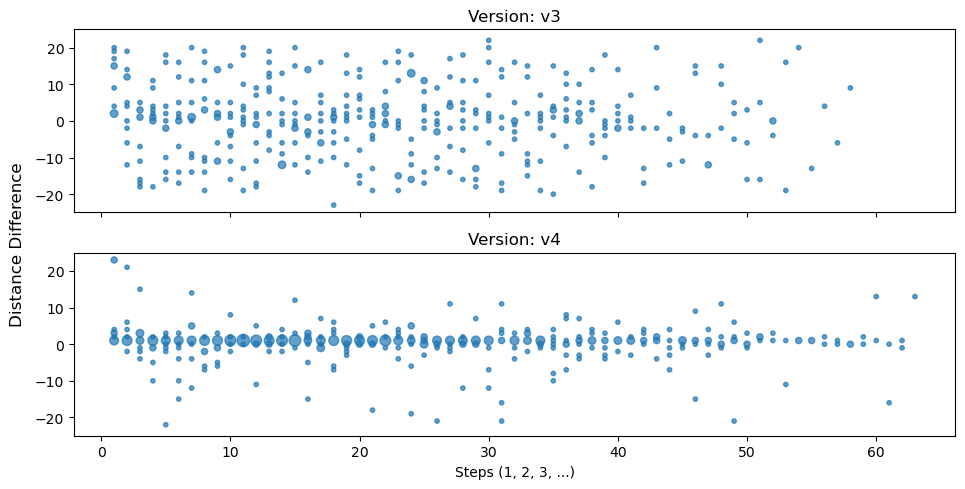
\includegraphics[width=0.75\textwidth]{content/image/distance/tmp_step-over-distance.png}
    \caption{Step-over Distance}
    \label{fig:step-over-distance}
\end{figure}

We focus our other two analysis given the statistical difference in the long survey. First, we examined whether participants moved more across the survey. Figure~\ref{fig:step-over-distance} visualizes the number of edits (radius) at each edit distance across all participants within the same experimental condition. The visualization highlights distinct participant behaviors: participants in the long text interface moved up and down with edit distances scatter with distinct values, whereas participants using the two-phase interface moved locally, making most edits nearby. Our hierarchical regression bayesian model (detailed in Appendix XX) that estimated a linear predictor of voting distances with the interface and individual users showed a statistical difference (report stats here) in variance with a large effect size confirming our belief. This indicates that participants, over the course of the survey, is making adjustments within close proximity of their previous edits in the long two phase interface compared to the static interface where participants are moving up-and-down. 

\begin{figure}[ht]
    \centering
    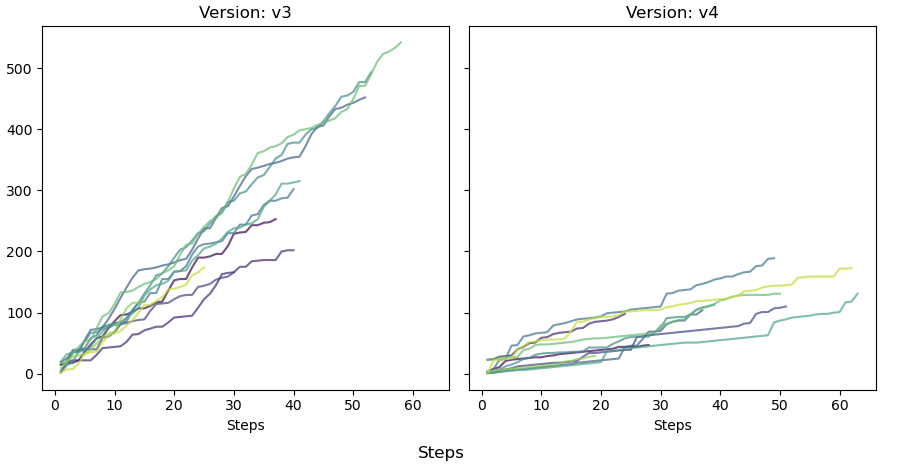
\includegraphics[width=0.75\textwidth]{content/image/distance/sum_dist.png}
    \caption{Cumulative Edit Distance}
    \label{fig:sum-distance}
\end{figure}

This reduction of the two-phase interface's effect on edit distance adds up, as Figure~\ref{fig:sum-distance} shows the cumulative edit distance over time, the slop of the two-phase interface is under the text interface. Our hierarchical regression bayesian model (detailed in Appendix XX) that estimated a linear predictor of cumulative distances with the interface, step, and individual users showed a statistical difference (posterior distribution has a mean difference of 4.8 in slope with a 94\% HDI of [4.1, 5.3] and a large effect size of XX) our belief.

These results provide evidence that the initial pass through the survey items, combined with the organizational phase, helped participants construct preliminary preferences, thereby reducing the need for large traversals between options. However, making nearby edits does not necessarily imply a narrow preference construction. 

Recall the differences in sources of cognitive load between the two experimental conditions: while two-phase interface participants made adjustments with nearby options, they experienced cognitive demand from preference construction due to broader considerations involving more options and higher-order values. Similarly, the qualitative results highlighted that long text interface participants constructed narrower preferences, yet their edit distance indicated that their movements covered more options. 

Notably, fewer participants (60\%, N=6) reported precise resource allocation in the long two-phase interface compared to 90\% in the long text interface. These results make it evident that two-phase interface participants were more focused on deliberating preferences than simply completing the survey. Furthermore, the ability to make localized adjustments while considering broader decisions suggests that participants constructed preliminary preferences during the grouping phase, allowing them to focus on deciding their votes. 

Thus, the difference in edit distance not only demonstrated that the interface reduced the need for participants to move across the survey but also highlighted that the two-phase interface enabled participants to stay more deeply engaged with the survey options and the preference construction task, particularly in the long survey.



% Physical demand refers to the physical effort required to complete a task, such as physical exertion or movement. The two-phase interface experienced higher physical demand from increased mouse usage.
